\documentclass{article}
\usepackage{graphicx}
\usepackage{mhchem}
\usepackage{tikz}
\usepackage{pgfplots}
\usepackage{filecontents}
\usepackage[T1]{fontenc}
\usepackage[utf8]{inputenc}
\usepackage[english, russian]{babel}

\graphicspath{ {./data/} } 

\title{Исследование явления осмоса на базе лабораторного стенда и расчёт зависимостей}
\author{Нестеров И.Д.}
\date{}

\begin{document}
    \selectlanguage{russian}
    \maketitle
    \tableofcontents
    \newpage

    \addcontentsline{toc}{section}{Введение}
    \section*{Введение}

        \hspace*{4mm}\textbf{\textit{Цель работы:}} Ознакомиться и научиться проводить исследования осмотических
        процессов в частности провести расчёты осмотического давления и осмотического потока, используя законы Фика.
        
        \addcontentsline{toc}{subsection}{Осмос}
        \subsection*{Осмос}
            \hspace*{4mm}\textit{Осмос} – частный случай \textit{диффузии}. Другими словами, это диффузия воды
            через полупроницаемую мембрану вниз по градиенту концентрации, когда
            растворенное вещество не может диффундировать через мембрану, а вода может,
            если мембрана проницаема для воды, но не для растворенного
            вещества. Вода будет выравнивать свою собственную концентрацию путем
            диффундирования в сторону с более низкой концентрацией воды.

            \begin{itemize}
                \item Вода считается универсальным растворителем -
                она связывает и растворяет полярные или заряженные
                молекулы (растворённые вещества)

                \item Поскольку растворённые вещества не могут
                проникнуть через клеточную мембрану без посторонней
                помощи, вода будет перемещаться, чтобы уравнять оба
                раствора

                \item При более высокой концентрации растворённого
                вещества в растворе меньше свободных молекул воды,
                поскольку вода связана с растворённым веществом
            \end{itemize}

            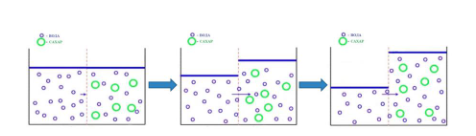
\includegraphics[width=0.9\textwidth]{Osmos.png}
        
        \newpage
        \addcontentsline{toc}{subsection}{Осмотическое давление}
        \subsection*{Осмотическое давление}
            \hspace*{4mm}\textit{Осмотическое давление} можно определить как минимальное давление, которое необходимо
            приложить к раствору, чтобы остановить поток молекул растворителя через
            полупроницаемую мембрану (осмос). Это коллигативное свойство, которое
            зависит от концентрации частиц растворенного вещества в растворе. Поэтому, по
            Вант-Гоффу, для вычисления осмотического давления можно воспользоваться
            уравнением Менделеева-Клапейрона:

            \begin{equation}
                P = \frac{m}{MV} \* RT = CRT    
            \end{equation}
            
            где C – молярная концентрация растворенного вещества в растворе, R –
            универсальная газовая постоянная, Т – температура, m – масса растворенного
            вещества, V – объем раствора, M – молярная масса растворенного вещества.

        \addcontentsline{toc}{subsection}{Осмотический поток}
        \subsection*{Осмотический поток}
            \hspace*{4mm}Для расчёта потока используем стандартную формулу для диффузного потока, однако с учетом того, что осмос
            является односторонним процессом диффузии, где движущая жидкость является
            вода, интерпретируя закон Фика под эту цель.

            \begin{center}
                Первый закон Фика:

                \begin{equation}
                    J = -D\frac{dC}{dx}    
                \end{equation}
            \end{center}
            
            где $D$ - коэффициент диффузии, $\frac{dC}{dx}$ - градиент концентрации
            вещества. \\

            %\hspace*{4mm}Коэффициент диффузии можно рассчитать как: 

            %\begin{equation}
            %    D = \frac{\Delta{V} \cdot \rho_{\ce{H2O}}}{M_{\ce{H2O}} \cdot S \cdot t}
            %\end{equation}

            %где $\Delta{V}$ - какой-то объём,
            %$\rho_{\ce{H2O}}$ - плотность воды, $M_{\ce{H2O}}$ - молярная масса воды,
            %$S$ - площать сечения капилляра, $t$ - время чего-то. \\

            %\hspace*{4mm}Подставив (3) в (2) и немного пренебрегая точностью расчётов,
            %получим уравнение для осмотического потока:

            %\begin{equation}
            %    J = -\frac{\Delta{V}\cdot\rho_{\ce{H2O}}\cdot|C_1 - C_2|}{M_{\ce{H2O}} \cdot S \cdot t \cdot L}
            %\end{equation}

            %где $L$ - толщина фланца.


    \newpage
    \addcontentsline{toc}{section}{Ход работы}
    \section*{Ход работы}

        \addcontentsline{toc}{subsection}{Растворы}
        \subsection*{Растворы}
            \hspace*{4mm}Было приготовлено два раствора \ce{CuSO4*5H2O} с разными концентрациями.
            Концентрация первого раствора составляла 10\%, второго - 20\%.


        \addcontentsline{toc}{subsection}{Установка}
        \subsection*{Установка}
            \hspace*{4mm}Для наблюдения и демонстрации осмотических процессов идеально
            подходит камера для осмоса и электрохимии. В обычной форме
            устройство имеет две стеклянные концевые камеры и двух резиновых
            уплотнительных колец, соединенных с помощью фланцевого держателя. Все
            камеры располагают стеклянную короткую трубку с резьбой GL25, на которую
            можно накрутить винтообразную крышку с кольцом уплотнения (25/8 мм).
            Экспериментируя с осмосом, стеклянные капиллярные трубки вставляют в эти
            соединительные крышки. \\
        
            \includegraphics*[width=0.8\textwidth]{tools1.png} \\

            \hspace*{4mm}Чтобы собрать двухкамерное устройство,
            Необходимо расположить подходящую полупроницаемую мембрану,
            изготовленную из целлофана, между двумя уплотнительными кольцами, а затем
            скрепить вместе две камеры прямоугольный зажимом, вместе с
            уплотнительными кольцами. \\

            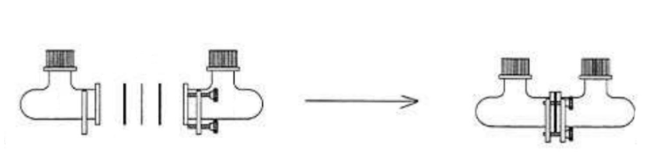
\includegraphics[scale=0.65]{tools2.png} \\

            \begin{center}
                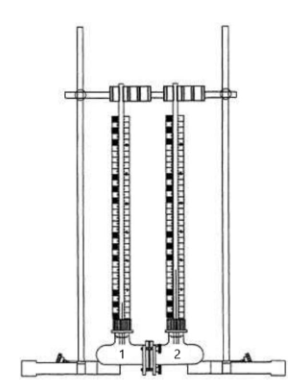
\includegraphics[scale=0.8]{tools3.png}
                \vspace*{4mm}
            \end{center}

            Характеристики компонентов:

            \begin{itemize}
                \item Внешний диаметр камеры: $D_o = 3.4$ см
                \item Внутренний диаметр камеры: $D_i \approx 3$ см
                \item Диаметр фланца: $D_o = 4.7$ см
                \item Толщина фланца: $d_o = 1$ мм
                \item Длина сегмента: $L \approx 90$ мм
                \item Высота: $H \approx 85$ мм
                \item Объём одного сегмента: $V \approx 65$ мл
            \end{itemize}
            \newpage

        \addcontentsline{toc}{subsection}{Наблюдения}
        \subsection*{Наблюдения}
            \hspace*{4mm}После сбора установки и начала эксперимента каждые 5 минут производились измерения высоты
            столбцов с растворами. \\

            Динамика высоты жидкости в первом сосуде, в котором концентрация составляла 10\%:
            \vspace*{8mm}

            \begin{tikzpicture}
                \begin{axis}[scale only axis,
                        ylabel=$h$,
                        xlabel=$t$,
                        xmax=35,
                        ymin=15, ymax=17,
                        xtick={0,5,...,30},
                        ytick={15.2,15.4,...,16.6},
                        axis lines=middle,
                        grid=both   
                    ] 
                    \addplot[only marks] table [col sep=comma] {./data/experiment1.csv};
                \end{axis}
            \end{tikzpicture}
            \newpage

            Динамика высоты жидкости во втором сосуде, в котором концентрация составляла 20\%:
            \vspace*{8mm}

            \begin{tikzpicture}
                \begin{axis}[scale only axis,
                        ylabel=$h$,
                        xlabel=$t$,
                        xmax=35,
                        ymin=17, ymax=21,
                        xtick={0,5,...,30},
                        ytick={17.5,18.0,...,20.5},
                        axis lines=middle,
                        grid=both   
                    ] 
                    \addplot[only marks] table [col sep=comma] {./data/experiment2.csv};
                \end{axis}
            \end{tikzpicture}
            \newpage

    \addcontentsline{toc}{section}{Обработка данных}    
    \section*{Обработка данных}
        \hspace*{4mm}В соответствии с формулой (1) были вычислены значения осмотического давления
        в течение эксперимента. \\

        Зависимость осмотического давления от времени отражена на графике ниже.

        %\begin{tikzpicture}
        %    \begin{axis}[scale only axis,
        %            axis lines=middle,
        %            grid=both
        %        ]
        %        \addplot[only marks] table
        %    \end{axis}
        %\end{tikzpicture}

    \addcontentsline{toc}{section}{Результаты и Выводы}
    \section*{Результаты и Выводы}


\end{document}